\chapter{Conclusions}
\label{ch:conclusions}
In the preceding chapters, we have focused on microsatellite instability and tumor heterogeneity. First, we introduced a new algorithm, MANTIS, for quantifying the extent of MSI in a tumor. We applied this algorithm to a large cohort of over 11,000 tumors from 39 types of cancer, and found that MSI can occur within at least a small proportion of many cancer types. To study tumor heterogeneity, we inferred tumor subclones and their evolutionary phylogeny in cases of cholangiocarcinoma, interdigitating dendritic cell sarcoma, and small cell lung cancer. Finally, we integrate these concepts in a cohort of patients with MSI-H metastatic cancer, and assess microsatellite changes within tumor subclones.

\section{Implications}
In all of these studies, we have seen the value of next-generation sequencing to provide insights into cancer biology and behavior. NGS becomes particularly powerful when applied at scale, whether broadly across large cohorts of patients, and/or at depth via sequencing of multiple samples from a patient. This provides opportunities to compare and contrast samples and patients, and to identify rare features present only in ``subsets of subsets'' of human cancer. For instance, we were able to identify the 4.3\% incidence of MSI in adrenocortical carcinoma only because of analysis of a large cohort (n=92) of ACC samples (Section~\ref{ssec:msilandscape:landscape_results}). Identifying subclones is valuable in its own right, and tools such as Sclust exist to detect subclones in single samples \cite{cun2018}. However multi-sample sequencing is necessary to more fully study subclones by inferring subclonal phylogeny \cite{tarabichi2021}, as multiple different combinations of subclones are needed. The continual decline in NGS costs (Section~\ref{ssec:intro:seq_beginnings}) along with the growth of cloud-based bioinformatics services \cite{banibaker2020} will further ease large-scale sequencing in the future.

Most notable in our investigation of MSI was our identification of a ``long tail'' of cancer types with infrequent MSI. Until this study \cite{bonneville2017} was published in \textit{JCO Precision Oncology} in 2017 along with others in the same journal issue \cite{middha2017,kok2017,klempner2017,haraldsdottir2017}, MSI had typically been thought of as essentially restricted to colorectal and endometrial cancers due to their association with Lynch syndrome (with the exception of case reports in other cancer types) \cite{lynch2015}. Today, MSI testing is increasingly deployed in a wider variety of cancer types \cite{eldeiry2019}, and it is included within several commercial genomic tests including FoundationOne \cite{trabucco2019} and Guardant360 \cite{willis2019}. Analysis of large, mixed cohorts has the potential to identify additional examples of genetic markers and features which may be present in a wider variety of cancers than previously thought. Such findings may expand the scope of patients who may benefit from therapies which leverage genetic markers, including immunotherapy for MSI (and other hypermutated tumors) and targeted inhibitors for kinase mutations and fusions.

We have presented four detailed studies of tumor heterogeneity, involving identification of cancer cell subclones, estimation of subclonal phylogeny, and various ancillary analyses. The concept of subclones provides a general framework for approximating tumor heterogeneity and microevolution which is applicable to a wide variety of cancer types and easily accessible to researchers and clinicians. We demonstrate that subclones can model the emergence of drug resistance mutations such as \textit{FGFR2} N549H to pemigatinib (Section~\ref{ssec:240:autopsy_results}) and \textit{AR} mutations to a variety of antiandrogens (Section~\ref{ssec:msiclones:clone_results}). Through NGS and subclonal analysis we were also able identify candidate mechanisms of hypermutation (Section~\ref{ssec:303:clone_results}), and to characterize examples of brain and prostate sanctuary sites. Furthermore, we show that the framework of subclones can be extended to temporally order mutations even within the same subclone (Section~\ref{ssec:240:mutational_ordering}), to retrospectively identify subclones in circulating tumor DNA (Section~\ref{ssec:sclc:ctdna_clones}), and to assess subclonal microsatellite distributions within heterogeneous tumor samples (Section~\ref{ssec:msiclones:subclonal_msi}).

Both MSI and subclonal evolution are examples of cancer as a dynamic process. Mismatch repair deficiency generates indel mutations with repeated cell divisions (Section~\ref{ssec:intro:mutation}), and sequencing of microsatellites (including analysis with tools such as MANTIS) provides a snapshot of accumulated MSI\@. Subclones reveal the evolutionary history of subclones observed in the tumor samples analyzed, often including ancestral clones which may have become extinct at the time of sampling. The IDCS, SCLC, and MSI-H cases in particular reflect the dynamic nature of cancer evolution due to their hypermutation, which provides many mutational events for study. From multiple time point sequencing (Section~\ref{ssec:msiclones:clinical_histories}), we identify shifts in tumor mutation and subclonal composition over time. In our analysis of subclonal MSI, we show that despite the stochastic nature of MMRd-driven mutations, they are inherited as are other mutations in subclones. Improved understanding of cancer mutational dynamics has the potential to improve cancer treatment by allowing proactive as well as reactive changes in therapy, and tailoring of regimens toward targets present in greater proportions of cancer cells \cite{hiley2014}.

\section{Future Directions}
In our study of 11,138 cancer cases, we found MSI in unexpected cancer types. As sequencing projects continue to expand, additional insights can be mined from growing data sets. Currently, there is a push to expand not only the breadth of sequencing but the depth, with recent whole genome sequencing projects highlighting the scalability of NGS \cite{cieslik2020}. Yet genomic sequencing fails to fully capture the complexity of cancer genetics, given the complexity of epigenetic factors such as DNA methylation and histone modification and the massive regulome of transcriptome factors (Section~\ref{ssec:intro:dna_function}). In addition to current and future large-scale RNA-seq studies, large-scale epigenetic studies are needed to provide such views of cancer. NGS-based technologies such as ChIP-exo (chromatin immunoprecipitation with exonuclease) \cite{rhee2012} and HT-ChIP (high-throughput ChIP) \cite{blechergonen2013} provide methods to survey modified histones and transcription factor activity, and their application to larger cancer cohorts has the potential to introduce another dimension to cancer landscape studies.

Another useful 'omics avenue is metabolomics \cite{li2017}, which studies levels of cell metabolites. Metabolomics studies typically utilize NMR and mass spectrometry to evaluate the abundance of small to medium-sized molecules (\textless{}~1.5~kDa) in cells and tissues \cite{wishart2007}. Though metabolomics is distinct from genomics, the metabolites which it studies are directly involved in cancer cell function and phenotype (versus DNA being a source of information). Large-scale metabolomics studies, in conjunction with genomics studies, can provide additional insights into the biochemical distinctions among cancers and additional context of the effects of mutations and other genomic alterations. Also important is proteomics \cite{aslam2017}, the study of the protein landscape of cells and tissues. The protein landscape is likely even more complex than the genomic landscape due to the enormous variety of protein interactions and post-translational modifications, yet with this complexity comes potential for finer-grained understanding of cancer biology.

Key to enhancing 'omics studies will be improved data integration. Despite the emergence of multi-omics projects such as The Cancer Genome Atlas \cite{tcgageneric}, which includes exome and transcriptome sequencing, methylomics (via microarray) and proteomics (via RPPA, reverse-phase protein array), today's studies struggle to correlate and compare 'omics studies of different modalities \cite{ulfenborg2019}. This will require substantial further research, particularly in bioinformatics and statistics due to the complementary but distinct nature of each platform \cite{subramanian2020}. Advances in machine learning, particularly deep learning, may provide a path for improved multi-omics integration to enable increased leverage of the multiple perspectives offered by these high-throughput methods \cite{nicora2020}. Integration may also extend to clinical and demographic covariates.

Rapid research autopsy is a powerful method to obtain multiple, high-quality, abundant tumor samples. However there are currently only about 24 autopsy programs in operation worldwide \cite{robb2021}, and establishing new programs poses substantial logistical challenges \cite{bacon2020}. Furthermore, the substantial majority of research autopsy programs focus on specific types of cancer. Therefore, increased collaboration between autopsy centers, perhaps a multi-center network, would allow additional research groups to benefit from access to autopsy tumor samples and draw further insights from the gift of each patient's donation.

Investigation of subclones also suggests multiple future directions. Implementing computational methods and pipelines for subclonal analysis is technically challenging \cite{tarabichi2021} and typically the domain of expert bioinformaticians. Greater involvement of basic scientists, clinicians, UI/UX professionals, cloud computing, and industry is necessary to lower the technical barriers to identifying and studying tumor subclones, and in turn to facilitate subclonal studies on a broader scale with larger cohorts \cite{wang2019}. In addition to larger cohort sizes, improved methods for comparing phylogenies are needed. Some methods such as phyC \cite{matsui2017} and GraPhyC \cite{govek2018} exist which map trees into a vector space to permit usage of clustering algorithms. However patient samples are typically highly variable, for instance two separate autopsies will yield different tumor sites and tissue quality. Additional work is necessary to evaluate the robustness of subclonal inference to differing experimental and clinical conditions, which will also facilitate improved meta-analyses of multiple cohorts from multiple institutions.

Subclonal models have significant potential for further extension. We quantified subclones in ctDNA in Chapter~\ref{ch:sclc}, however these subclones were defined by the autopsy samples. Development of methods that utilize ctDNA alongside solid tumor samples in subclonal phylogenetic inference would bring the advantage of establishing time points by which certain mutations were present, providing phasing information to more accurately order mutational events in the tree. Single-cell sequencing \cite{navin2011} provides a powerful orthogonal means of studying heterogeneity, offering higher resolution at the cost of less comprehensive sampling. Hybrid approaches could bridge this gap, for instance by ``splitting'' certain subclones as well as also providing phasing information.

Generally, subclonal analyses generate subclonal populations, and a phylogenetic tree with sets of mutations assigned to each edge. Even when these analyses are extended to yield ordered lists rather than sets, they can at best provide a relative ordering of mutations rather than an absolute chronology. This ultimately limits biological and clinical interpretability, as it is difficult to correlate mutations with specific events in the patient's disease course. Some recent heterogeneity software packages such as PhylogicNDT \cite{leshchiner2019} incorporate time point data of input tumor samples and utilize this to computationally estimate paths of tumor cell migration, but due the clinical difficulties of obtaining multiple sequential biopsies the available time points are typically sparse. Furthermore, mutation rates in cancer are highly nonlinear due to the effects of different environmental stressors and changes in cancer cells' DNA replication and repair proficiency. A need remains for a bioinformatics approach that explicitly models time in phylogeny, for instance to estimate the months post-diagnosis that a key mutation was acquired. Such an approach could conceivably utilize a differential equations-based approach \cite{steely2013} to model cancer kinetics. In addition, bioengineered `lineage tracers' have been recently developed, for instance utilizing CRISPR/Cas9 editing to induce mutations at a known constant rate at specified genomic locations \cite{quinn2021}. By introducing mutations whose timing can be well estimated, lineage tracers have the potential to facilitate direct interrogation of mutational dynamics in model systems, and their predictability also facilitates accurate subclonal phylogenetic inference.

\begin{figure}
    \centering
    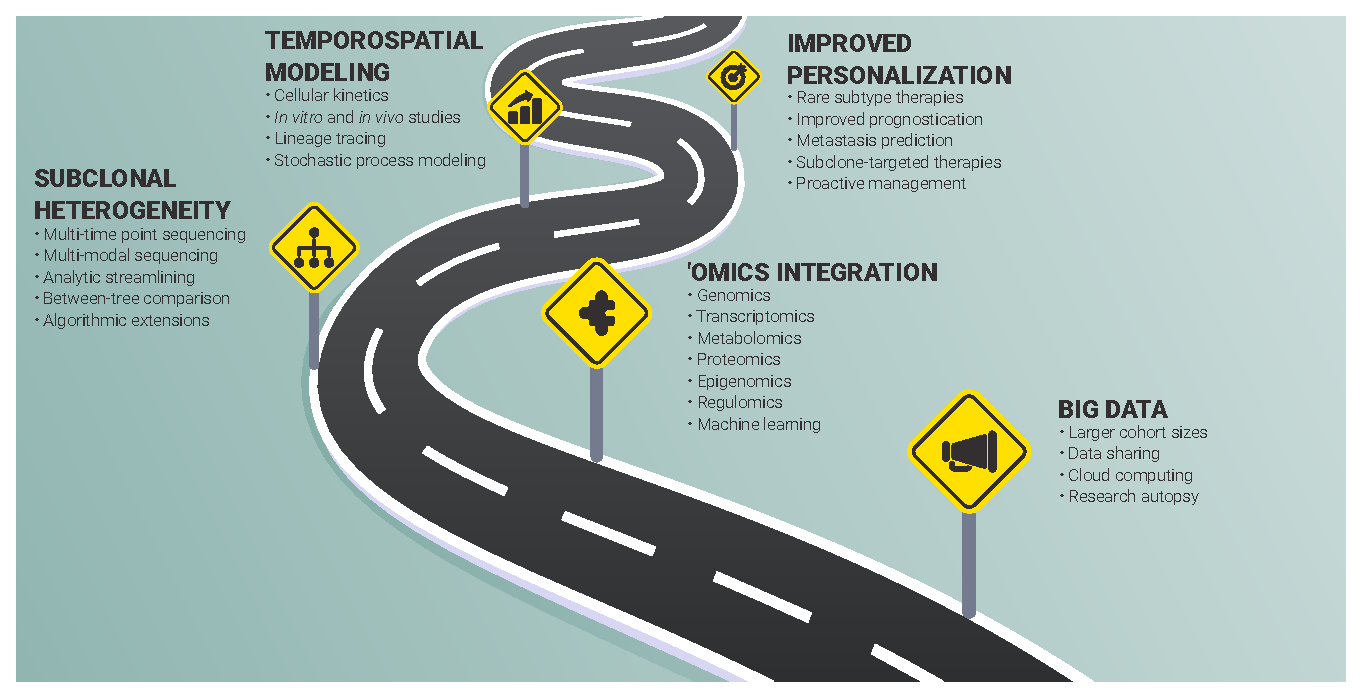
\includegraphics[width=\textwidth,keepaspectratio]{images/conclusion/future_roadmap}
    \caption[Roadmap of future directions.]{Roadmap of future directions which emerge from view of cancer as a dynamic process. Leveraging ``Big Data'', such as through large, multi-center cohorts, will support integration of multiple 'omics methods, facilitated by improved statistical models and machine learning. Building upon concepts of subclonal heterogeneity will further reveal the evolutionary histories of cancer, which can be coupled with temporospatial modeling of heterogeneity and cancer mutation to permit improved prediction of a patient's cancer progression and clinical course. This in turn will allow further personalization of cancer management and treatment, leading to improved patient outcomes. Figure is derived from ``Outstanding Road Map Vectors'' by Rizki Kurniawan (\href{https://www.vecteezy.com/vector-art/211642-outstanding-road-map-vectors}{Vecteezy.com}).}
    \label{fig:conclusions:future_roadmap}
\end{figure}
Lipinski \textit{et al} propose a view of cancer evolution as a continuum of deterministic and stochastic processes which unfold throughout the disease course \cite{lipinski2016}. Furthermore, they utilize the concept of the ``predictability horizon'', essentially the maximal accuracy at which current methods can predict and model tumor evolutionary dynamics and clinical correlates (such as treatment response and survival). Though this horizon remains clouded at present, in this work we have demonstrated the ability of large-scale NGS analysis and enhanced subclonal modeling to provide retrospective but clinically meaningful insights into temporal tumor evolution. With further investigation and algorithmic enhancements (Figure~\ref{fig:conclusions:future_roadmap}), it is our hope that the cancer predictability horizon will progressively expand into the future.

%cancer as process

%possible future directions, MSI related: further surveys of mutational patterns (like orien hypermutation project), retrospective analysis based on treatment performance
%possible future directions for subclones: ctdna, predictive models, direct modeling of time (cite phylogicndt), comparisons across trees
%subclones potentially useful even if not as precise as single-cell; Although single-cell sequencing offers higher resolution than bulk NGS-based strategies, subclones are (other possible extensions)
%msi clones (extension to previous subclonal analyses) demonstrates untapped potential for subclonal models
%possible future directions: other combinatorial problems, hybrid single-cell/bulk (also would have potential to permit subclonal rna, which is otherwise underspecified)
    %subclonal rna a ``holy grail'', but mathematically underspecified with an approach like msi clones
    %improved ctdna integration (clones over time, and improved accuracy of tree by phasing)
    %in vivo model systems, i.e. 10.1126/science.abc1944
%for last paragraph, about cancer as process. Base on https://pubmed.ncbi.nlm.nih.gov/31162540/, https://www.ncbi.nlm.nih.gov/pmc/articles/PMC4756277/
    
%TODO: ref SCLC as appropriate!
